% Введение.
\newpage
\section*{Введение}                      % выключить номер введения
\addcontentsline{toc}{section}{Введение} % но добавить его в оглавление

Высокопроизводительные вычисления являются неотъемлемой составляющей научных исследований, промышленных разработок и бизнеса.
Использование высокопроизводительных вычислительных систем \cite{GOST57700HPC} находит широкое применение во всех сферах деятельности человека.

% а) переход к передовым технологиям проектирования и создания высокотехнологичной продукции.
Суперкомпьютерные вычисления являются основой для развития передовых технологий проектирования и создания высокотехнологичной продукции.
В частности суперкомпьютерные вычисления применяются в авиационной и космической промышленности \cite{Kornev2021SuperAvio}, автомобилестроении \cite{Wang2020SuperAuto}, проектировании морского и железнодорожного транспорта \cite{Nikitin2018SuperShip,Solovyev2013SuperTrains}, турбин \cite{Duben2022SuperTurbine} и других высокотехнологичных изделий.
Важную роль суперкомпьютеры играют при проектировании образцов вооружения, в частности военной техники и боеприпасов \cite{Ageeva2023SuperMilitary}.
Также суперкомпьютерные вычисления незаменимы при разработке новых материалов, для изучения свойств которых требуется проводить точное атомистическое моделивование структур, состоящих из миллиардов отдельных атомов \cite{Wang2025SuperMolDyn}.

% б) переход к экологически чистой и ресурсосберегающей энергетике, повышение эффективности добычи и глубокой переработки углеводородного сырья, формирование новых источников энергии, способов ее передачи и хранения.
В энергетической сфере высокопроизводительные вычисления применяются для моделирования объектов генерации электроэнергии, включая атомные станции \cite{Cancemi2025SuperNuc} (в совокупности с процессами внутри ядерных реакторов \cite{Zhang2025SuperNuclear}), ветряные и приливные генераторы \cite{Quint2025SuperWind,Parrado2024SuperTidal}.
Детальное моделирование месторождений углеводородного сырья позволяет повысить эффективность добычи \cite{Usmanov2024SuperPlast}, а создание цифровых моделей месторождений и систем транспортировки \cite{Didenko2023SuperOil} приводит к снижению потерь и обеспечивает прозрачность полного жизненного цикла, начиная с добычи сырья и заканчивая реализацией конечного топлива потребителю.

% в) переход к персонализированной, предиктивной и профилактической медицине, высокотехнологичному здравоохранению и технологиям здоровьесбережения, в том числе за счет рационального применения лекарственных препаратов.
Использование больших вычислительных систем позволило извлекать качественно новые данные из точного моделирования крупных органических молекул и их ансамблей \cite{Teplukhin2009SuperBigMolec}.
Во время борьбы с пандемией COVID-19 суперкомпьютерные вычисления играли передовую роль в изучении вируса и разработке вакцины \cite{Colonnelli2021SuperCovid}.
Обработка с помощью искусственного интеллекта больших массивов медицинских данных, включая истории болезней, медицинские анализы и снимки \cite{Ri2024SuperXRay}, в совокупности с геномными исследованиями в настоящее время знаменует переход к персонализированной медицине \cite{Kishore2024SuperPrecMed}.

% г) переход к высокопродуктивному и экологически чистому агро- и аквахозяйству, разработку и внедрение систем рационального применения средств химической и биологической защиты сельскохозяйственных растений и животных, хранение и эффективную переработку сельскохозяйственной продукции.
Компьютерное моделирование активно используется в растениеводстве и животноводстве для повышения эффективности выработки продовольствия.
Сюда входит целый спектр применений, начиная от селекции растений и животных \cite{Ahmetshina2020SuperSelection}, мониторинга их здоровья \cite{Mourant2018SuperEpi}, разработки удобрений и кормов \cite{Irfan2016SuperFert} и заканчивая планированием графиков разведения животных и выращивания сельскохозяйственных культур \cite{Zhang2021SuperFertPlan}.

% д) противодействие техногенным, биогенным, социокультурным угрозам, терроризму и экстремистской идеологии, деструктивному иностранному информационно-психологическому воздействию, а также киберугрозам и иным источникам опасности для общества, экономики и государства, укрепление обороноспособности и национальной безопасности страны в условиях роста гибридных угроз.
В связи со стремительным распространением цифровизации во всех областях современной жизни и ростом объема цифровых данных особую важность обретает задача обеспечения кибербеопасности и сохранности данных.
Злонамеренные действия в киберсреде потенциально могут привести к серьезным последствиям, включая финансовые потери, техногенные и экологические катастрофы.
Высокопроизводительные вычисления используются для исследования и созданиия новых инструментов информационной безопасности, в том числе с помощью технологий искусственного интеллекта и систем распределенного реестра \cite{Terziyska2024SuperCyber}.

% е) повышение уровня связанности территории Российской Федерации путем создания интеллектуальных транспортных, энергетических и телекоммуникационных систем, а также занятия и удержания лидерских позиций в создании международных транспортно-логистических систем, освоении и использовании космического и воздушного пространства, Мирового океана, Арктики и Антарктики.
Ввиду обширности территории России и неравномерности ее заселения и инфраструктурного обеспечения, необходимо создание интеллектуальных транспортных и телекоммуникационых систем для повышения уровня связности территории.
Суперкомпьютерные вычисления применяются для проектирования и развития систем железнодорожного и авиасообщения \cite{Juntana2022SuperFlight}, обеспечения логистики морских перевозок \cite{Yan2024SuperSea}, а также для создания глобальных компьютерных сетей \cite{Abramov2025SuperNets}.

% ж) возможность эффективного ответа российского общества на большие вызовы с учетом возрастающей актуальности синтетических научных дисциплин, созданных на стыке психологии, социологии, политологии, истории и научных исследований, связанных с этическими аспектами научно-технологического развития, изменениями социальных, политических и экономических отношений.
%Развитие цифровизации во всем мире затрагивает не только технические стороны жизни человека, но и социально-психологические аспекты.
%В настоящее время можно констатировать, что социально-психологический профиль человека практически полностью определяется по его цифровому следу.
%Это с одной стороны открывает возможности по моделированию социальных и политических процессов \cite{} на основе цифровых данных.
%С другой стороны, доступность цифровых данных создает уязвимости как отдельного человека, так и целых групп населения, поэтому такие угрозы также нужно %анализировать и парировать \cite{}.

% з) объективную оценку выбросов и поглощения климатически активных веществ, снижение их негативного воздействия на окружающую среду и климат, повышение возможности качественной адаптации экосистем, населения и отраслей экономики к климатическим изменениям.
Так как техногенное влияние человека на окружающую среду постоянно возрастает, то в настоящее время высокопроизводительные вычисления применяются для решения задач экологии.
В частности с помощью суперкомпьютерного моделирования и глобальных моделей проводятся климатические исследования \cite{Kulkarni2024SuperClimate}, исследования мирового океана \cite{Wei2024SuperOcean}, экосистем \cite{Rahman2024SuperSpecies} и оцениваются выбросы в окружающую среду и их последствия \cite{Ostromsky2024SuperAir}.

% и) переход к развитию природоподобных технологий, воспроизводящих системы и процессы живой природы в виде технических систем и технологических процессов, интегрированных в природную среду и естественный природный ресурсооборот.
В последнее время особый акцент в технологическом развитии делается на природоподобные технологии, основанные на воспроизведении систем и процессов живой природы.
Как правило, эти системы и процессы состоят из большого количества взаимодействующих элементов, которые требуют точного моделирования, что возможно только с использованием суперкомпьютеров.
К природоподобным направлениям, связанным с высокопроизводительными вычислениями, можно отнести разработку нейроморфных процессоров~\cite{Rhodes2019SuperNuero}, технологии синтеза и воспроизведения тканей и органов человека \cite{Wang2012SuperTissues}, топологическую оптимизацию в проектировании изделий и строительстве \cite{Fedchikov2024SuperBim} и другие направления.

% Суррогатные вычисления.
Широкое применение суперкомпьютерного моделирования в проектировании сложных технических систем связано с задачей выбора оптимальной конфигурации при большом количестве входных параметров.
По мере усложнения проектируемых систем и роста количества параметров возникла проблема дефицита вычислительных ресурсов, что привело к появлению концепции суррогатного моделирования \cite{Jiang2020Surrogate,Barcenas2023Surrogate,Catalani2024Surrogate}, то есть использования упрощенных суррогатных моделей, обученных на результатах суперкомпьютерного моделирования на ограниченных наборах данных.
Но даже использование суррогатного моделирования может лишь частично снизить потребность в вычислительных ресурсах и не умаляет актуальность проблемы эффективного их использования.

Приведенный выше, но далеко не полный перечень сфер применения высокопроизводительных вычислений отражает основные приоритеты научно-технологического развития Российской Федерации.
Развитие суперкомпьютерных технологий необходимо для обеспечения места России среди мировых технологических лидеров, поэтому вопросы создания и эффективного использования высокопроизводительных вычислительных систем являются крайне актуальными, особенно в условиях настоящего дефицита высокопроизводительных ресурсов в Российской Федерации \cite{Voevodin2021SuperRussia}.

% Расчеты в пространстве и на поверхности.
Наиболее ресурсоемкие научно-технические задачи, связанные с суперкомпьютерными расчетами, представляют собой моделирование различных физических процессов в трехмерном пространстве.
К таким задачам относятся моделирование процессов газовой динамики \cite{Lobanova2023GeneralGas}, электромагнетизма \cite{Taboada2013GeneralElectro}, термодинамики \cite{Liu2020GeneralThermo} и многих других.
При этом вычисления проводятся, как правило, с использованием расчетных сеток, которые могут описывать, как область трехмерного пространства (объемные расчетные сетки \cite{Kudryavzeva2014GeneralVolumeMesh}), так и некоторую расположенную в трехмерном пространстве поверхность (поверхностные расчетные сетки \cite{Zheleznyakova2016GeneralSurfMesh}).

% Задачи на поверхностях.
К числу задач суперкомпьютерного моделирования на поверхностных расчетных сетках относятся задачи внешнего обтекания \cite{Mitin2020Flow}, течения пленки жидкости по поверхности \cite{Li2014Film}, обледенения поверхности \cite{Koshelev2020Ice,Sorokin2020Ice}.
При этом задача обледенения поверхности является комплексной, так как для получения адекватной картины ледообразования необходимо учитывать множество сопряженных процессов, включая обтекание тела, выпадение на поверхность влаги и ледяных кристаллов из окружающего потока \cite{Cui2023Impingement}, взаимодействие выпадающего вещества с поверхностью \cite{Cui2021Impingement}, течение жидкости по поверхности в виде тонкой пленки или отдельных нитей \cite{Alexeenko2013Ice}, теплопроводность на поверхности \cite{Domingos2015IceHeat}, а также через слой жидкости и льда \cite{Xin2013Ice} и многие другие процессы.
Также в процессе образования слоя льда меняется сама геометрия рассматриваемой поверхности, так как форма образовавшихся ледяных наростов существенным образом влияет на все связанные процессы, что приводит к необходимости перестроения расчетных сеток.

% Настоящая работа.
Настоящая работа посвящена оптимизации суперкомпьютерных вычислений для моделирования процесса обледенения поверхности, хотя результаты работы применимы и к другим предметным областям.
Вычисления по моделированию обледенения проводятся на поверхностных неструктурированных расчетных сетках, описывающих поверхность в трехмерном пространстве и способных изменять свою геометрию в процессе проведения расчетов, а также на объемных расчетных сетках, описывающих область пространства вокруг этой поверхности.

\paragraph{Актуальность темы} \

Задача моделирования обледенения летательных аппаратов является критически важной для обеспечения безопасности полетов \cite{Raj2020IntroIce}.
Изучение процессов формирования ледяных наростов имеет большую практическую значимость, так как характер и размер ледяных наростов существенно влияют на летные характеристики летательного аппарата.
Известны случаи, когда обледенение несущих частей и силовых установок летательных аппаратов приводили к авиакатастрофам с большим количеством человеческих жертв\footnote[1]{Катастрофа Ан-148 в Подмосковье в 2018 г., катастрофа DC-8 в Канаде в 1985 г., катастрофа Ту-134 под Минском в 1985 г., катастрофа MD-83 в Мали в 2014 г., катастрофа Ан-24 в Бугульме в 1991 г.}, что свидетельствует о важности этой задачи и востребованности результатов ее решения.
Требования и рекомендации к процессам проектирования, разработки и сертификации авиационных систем с учетом эксплуатации в режимах обледенения зафиксированы во многих нормативных документах\footnote[2]{14 CFR -- Part 25 (Appendix C, O), Part 29 (Appendix C), Part 33 (Appendix D); FAA AC 25-28; ARP 4754; ARP 4761; Р 4761; ISO 11076:2020; Doc 9640; FAA Report ADS-4; FAA Report RD-77-76; НЛГ БАС-СТ.}.

В пользу актуальности и востребованности исследований и разработок в области моделирования обледенения свидетельствует большое количество существующих и разрабатываемых программных пакетов для решения этой задачи.
Среди зарубежного программного обеспечения для моделирования процесса ледообразования лидером является пакет инженерного проектирования ANSYS (включающий в себя модули FENSAP-ICE, DROP3D, ICE3D) \cite{Martini2022IntroIce}.
Кроме него можно назвать и другие расчетные коды, например, LEWICE \cite{Shannon2019IntroIce}, AIPAC \cite{Domingos2015IceHeat}, ONERA \cite{Villedieu2014IntroIce}, TRAJICE \cite{Son2010IntroIce} и другие.
В России в настоящее время также разрабатывается набор алгоритмов и программного обеспечения для моделирования процесса ледообразования.
В их числе можно назвать разработку модуля iceFoam как части открытого программного обеспечения OpenFOAM \cite{Koshelev2020Ice}.
Среди коммерческих программных продуктов выделяется модуль IceVision в составе пакета FlowVision \cite{Sorokin2020Ice}, а также решение для моделирования ледяного покрова в составе пакета инженерного анализа ЛОГОС \cite{Galanov2021IntroIce,Galanov2021IntoIceLOGOS}.

Моделирование процесса ледообразования выполняется, как правило, на поверхностных расчетных сетках и состоит из отдельных макроитераций, каждая из которых проходит в два этапа.

На первом этапе итерационно выполняется расчет интенсивности нарастания льда в рамках отдельных ячеек расчетной сетки (интенсивность ледообразования может выражаться в массе накопленного льда в ячейке за временя макроитерации, в скорости нарастания высоты ледяного покрова в узле сетки и в других характеристиках).
Для вычисления интенсивности ледообразования в элементах расчетной сетки существует множество моделей ледообразования \cite{Bartkus2018IntroIce,Zhang2017IntroIce,Pena2016IntroIce}, в которых учитываются различные состояния льда, течение жидкой пленки по поверхности, тепловые потоки, выпадение на поверхность влаги, ледяных кристаллов и переохлажденных капель \cite{Wang2023IntroIce,Liu2022IntroIce}, различные механики плавления и срыва ледяных наростов \cite{Ruan2023IntroIce} и многие другие факторы. 

%\begin{figure}[ht]
%\centering
%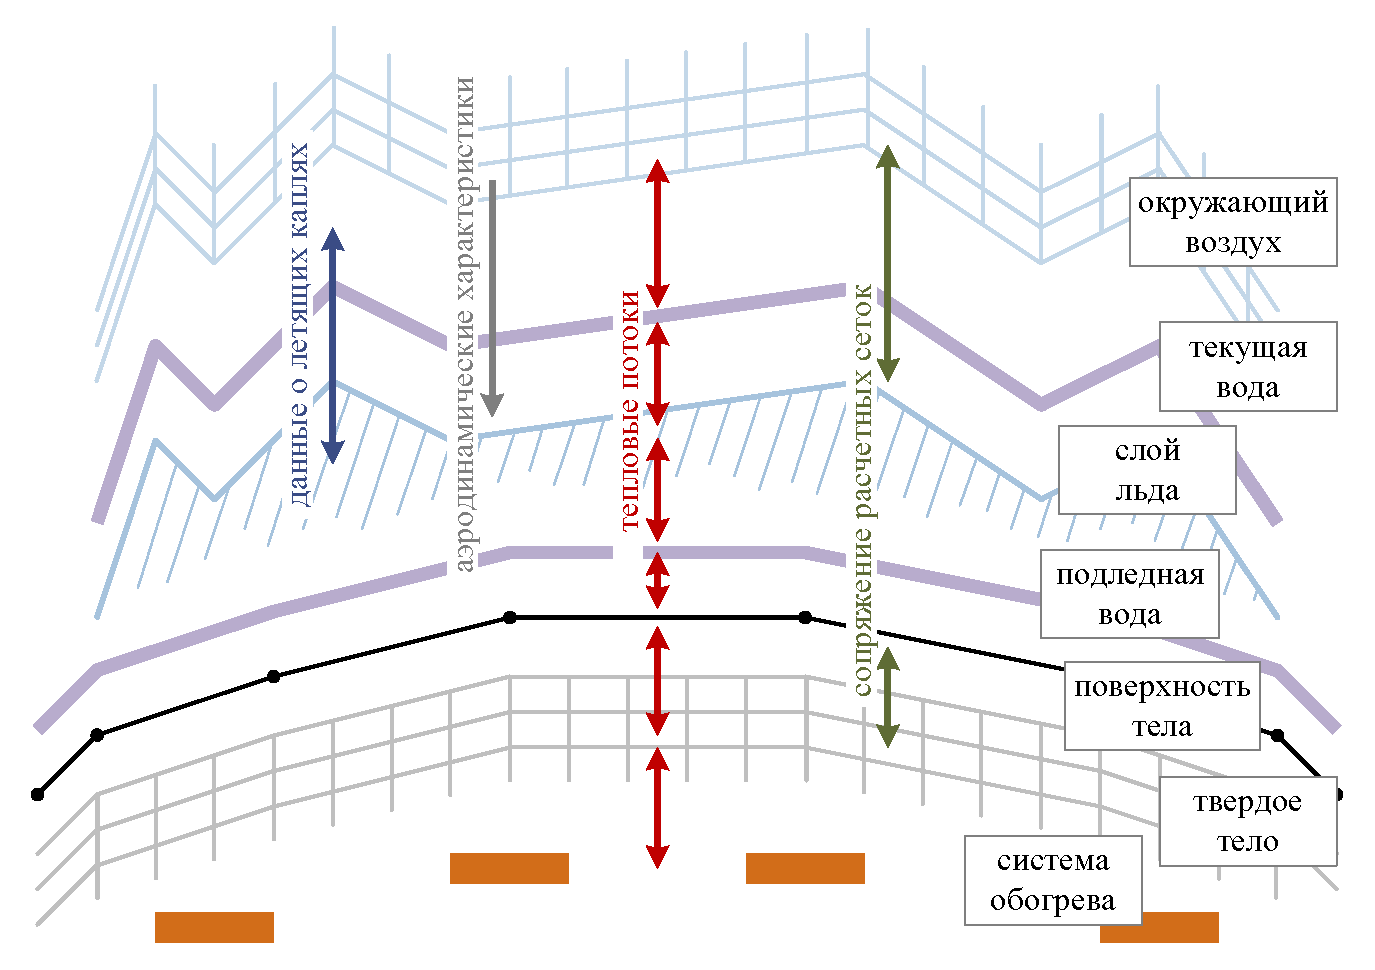
\includegraphics[width=1.0\textwidth]{pics/text_0/multi-scheme.pdf}
%\singlespacing
%\captionstyle{center}\caption{Многослойная модель ледообразования.}
%\label{fig:text_0_multi_scheme}
%\end{figure}

%Во время расчета первого этапа каждая ячейка поверхностной расчетной сетки представлена в виде сложной структуры, состоящей из следующих слоев, перечисленных снизу вверх: элементы системы обогрева внутри тела -- твердое тело -- слой находящейся подо льдом жидкости -- слой льда -- текущая по поверхности льда жидкость -- окружающее воздушное пространство (см. рис.~\ref{fig:text_0_multi_scheme}).
%В зависимости от используемой модели можно выделять и другие слои.
%Во время выполнения расчетов осуществляется обмен потоками вещества и тепла между отдельными слоями, а также между соседними ячейками.

На втором этапе моделирования ледяных наростов выполняется перестроение поверхности обледеневающего тела.
При этом перестроение должно выполняться таким образом, чтобы изменение объема рассматриваемого тела соответствовало вычисленному объему накопленного за время макроитерации льда на первом этапе.
После перестроения поверхностной расчетной сетки необходимо произвести пересчет поля скоростей вокруг нее, так как изменение геометрии поверхности существенным образом влияет на картину обтекания.
После пересчета поля скоростей моделирование процесса обледенения может быть продолжено.

Моделирование процесса ледообразования является крайне ресурсоемким процессом, включающем в себя не только выполнение вычислений на поверхностной расчетной сетке, но и постоянное перестроение поверхностной сетки и пересчет поля скоростей в окружающем пространстве.
Перестроение поверхностной расчетной сетки, адекватно описывающей геометрию образующихся ледяных наростов, должно отвечать критериям точности перестроения и устойчивости.
Возникновение дефектов сетки, таких как острые пики и изломы, трещины и впадины, самопересечения сетки, могут привести к аварийному завершению процесса расчета и необходимости его перезапуска, что приводит к дополнительному потреблению вычислительных ресурсов. 
Для выполнения моделирования образования ледяных наростов на значимом промежутке времени требуется использование существенных суперкомпьютерных ресурсов и применение методов для оптимизации вычислений на поверхностных и объемных расчетных сетках на всех уровнях распараллеливания: в модели с передачей сообщений, на общей памяти и на уровне отдельных инструкций.

\paragraph{Цели и задачи работы} \

\input text_goal.tex

\input text_tasks.tex

\paragraph{Методология и методы исследования} \

Математическую основу исследования составляют методы вычислительной геометрии, теории алгоритмов, теории графов, теории вероятностей.
Для замера эффективности использования суперкомпьютерных ресурсов применялись численные эксперименты на суперкомпьютерах Межведомственного суперкомпьютерного центра Российской академии наук и Национального исследовательского центра <<Курчатовский институт>>.

\input text_new.tex

\paragraph{Достоверность полученных результатов} \

Достоверность полученных результатов подтверждается экспериментами на суперкомпьютерах Межведомственного суперкомпьютерного центра Российской академии наук и Национального центра <<Курчатовский институт>> и практикой применения в программном модуле компьютерного моделирования процесса обледенения элементов авиационных силовых установок <<Кристалл>>.

\paragraph{Теоретическая и практическая значимость} \

\input text_theoretical.tex

Описанные в работе методы и алгоритмы апробированы на суперкомпьютерах Межведомственного суперкомпьютерного центра Российской академии наук и Национального центра <<Курчатовский институт>> и реализованы в рамках инструментов суперкомпьютерного моделирования, на которые оформлены 7 свидетельств о государственной регистрации программы для ЭВМ \cite{CertGoryachev2023Crys,CertGoryachev2020Crys,CertRybakov2021PrepUnstruct,CertRybakov2020PrepStruct,CertRybakov2024Surf,CertRybakov2023Mon,CertRybakov2019AVX}.
В частности, разработанные в рамках диссертации методы перестроения поверхностной неструктурированной расчетной сетки и устранения самопересечений, а также методы повышения эффективности суперкомпьютерных расчетов на ней нашли свое отражение в программном модуле компьютерного моделирования процесса обледенения элементов авиационных силовых установок <<Кристалл>> \cite{CertGoryachev2023Crys,CertGoryachev2020Crys}.

\input text_statements.tex

\input text_spec_passport.tex

\input text_conferences.tex

\input text_myown.tex

\input text_publications.tex

\input text_struct.tex

\input text_brief_content.tex
